% Modulo 1: Telescopios-Generalidades
% Objetivo: Proporcionar a los miembros del club la información fundamental de telescopios con énfasis en telescopios Newtonianos (reflectores), incluyendo historia, principios ópticos, ventajas y desventajas y aplicaciones básicas. 

\section{Introducción}

La palabra telescopio proviene del griego \foreignlanguage{greek}{τῆλε} (tēle, “lejos”) y \foreignlanguage{greek}{σκοπέω} (skopeō, “observar”); es decir, un instrumento utilizado para observar a lo lejos. Estos instrumentos ópticos permiten captar con mayor precisión y detalle una porción de la radiación electromagnética proveniente de cuerpos distantes.

Su invención y desarrollo han sido fundamentales para la observación y comprensión del universo. Gracias al telescopio, la humanidad ha podido explorar desde objetos cercanos como el Sol, la Luna, los planetas y sus satélites, y mucho más lejanos como nebulosas, cúmulos estelares y galaxias remotas (fig\ref{fig:telescopio_antiguo}).

% SUGERENCIA: incluir una imagen de un telescopio clásico apuntando al cielo nocturno.
\begin{figure}[H]
	\centering
	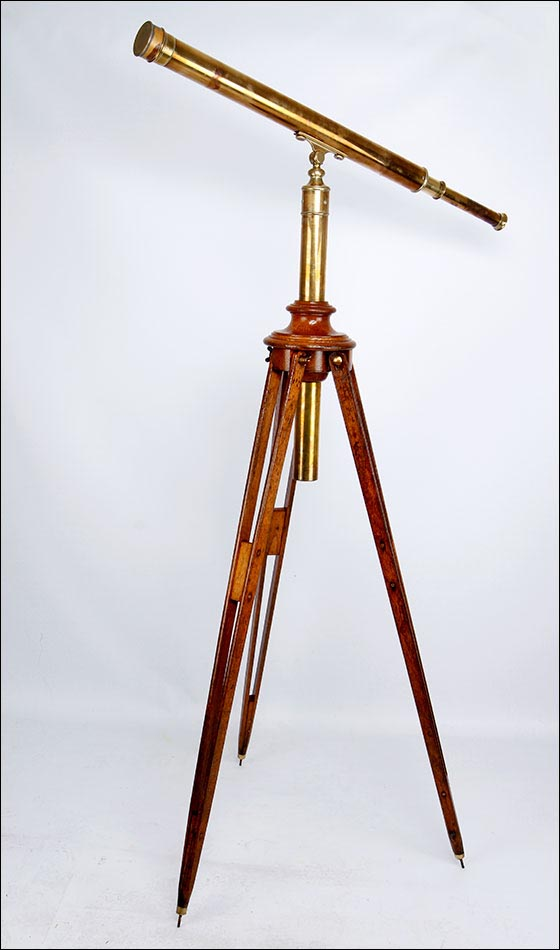
\includegraphics[width=0.6\textwidth]{images/telescopio_antiguo.jpg}
	\caption{Telescopio antiguo, aproximadamente de principios de los 1800.}
	\label{fig:telescopio_antiguo}
\end{figure}

Históricamente, la patente original de un telescopio refractor intentó ser patentada por Hans Lipperhey, un fabricante de lentes Holandés. La idea de utilizar dos lentes en un instrumento óptico se esparció por toda Europa, llegando así al conocimiento de Galileo Galilei, quién construyó una versión propia y la utilizó para observar el cielo nocturno. Así logró ver objetos invisibles al ojo humano, como las lunas de Júpiter y estrellas ubicadas en regiones aparentemente “vacías” del cielo.

La versión de Galileo permitía un aumento hasta de 8 veces, sin embargo sus primeros usos fueron en la industria militar, dando así una gran ventaja ante el enemigo. Pese a esto, Galileo también utilizó su descubrimiento para investigar el cielo nocturno.

Algunas de las observaciones del cielo que procedieron a su modificación del telescopio, Galileo consiguió pruebas certeras a favor de la teoría copernicana, que planteaba el sol como centro de todo, contraria a la geocéntrica, que planteaba la tierra como el centro del universo. 


\begin{figure}[H]
	\centering
	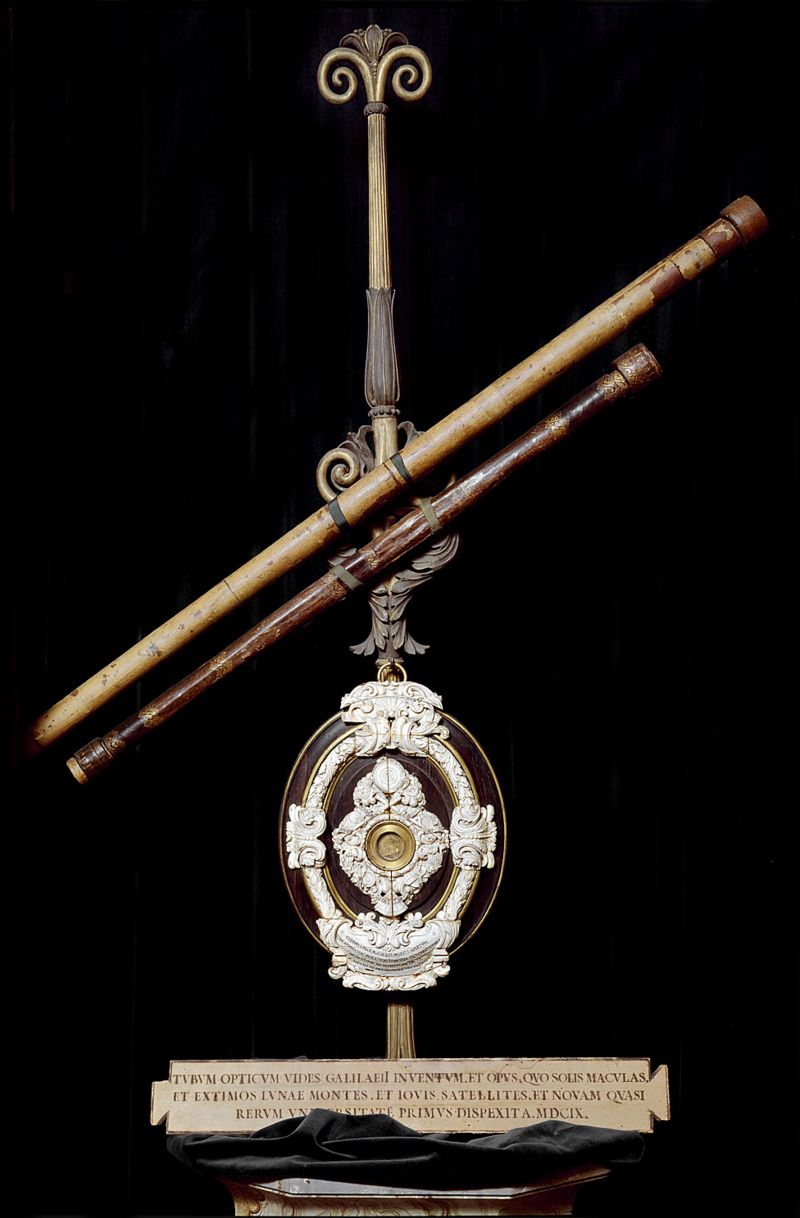
\includegraphics[width=0.6\textwidth]{images/telescopio_galileo.jpg}
	\caption{Versión modificada de telescopios tradicionales hecha por Galileo para poder captar mejor objetos lejanos.}
	\label{fig:telescopio_patente_galileo}
\end{figure}
% SUGERENCIA: insertar un video corto o animación de las lunas de Júpiter orbitando.
% También podría incluirse una ilustración de Galileo observando con su telescopio.

El término \textbf{telescopio} abarca una amplia variedad de dispositivos: radiotelescopios, telescopios infrarrojos y ultravioletas, así como \textbf{telescopios ópticos}. En este documento nos enfocaremos en estos últimos, que son los más comunes y accesibles, ideales para introducirse al mundo de la observación astronómica.

Esta guía forma parte del minicurso organizado por la Comisión de Creación de Telescopios del Capítulo de Óptica de Yachay Tech, realizado en abril de 2024.

\subsection*{Breve historia del telescopio}

El registro más antiguo sobre la existencia de uso de un telescopio refractor corresponde a una patente solicitada por Hans Lippershey, desde Holanda, en el siglo XVII, pese a que no se la otorgó el diseño del instrumento se popularizó alrededor de Europa, y fue en 1609 cuando Galileo Galilei lo empleó con fines astronómicos para observar el cielo, marcando un hito en la historia de la ciencia. Esto debido a que sus resultados respaldaban la teoría heliocentrista y se iba en contra lo aceptado de la época, la teoría geocéntrica, donde se asume que la tierra es el centro del universo, donde los planetas, la luna y las estrellas giran alrededor nuestro. Galileo no sólo tomaba nota de sus observaciones, sino que también creaba ilustraciones de sus hipótesis (fig \ref{fig:ilustracion_luna_galileo_1610}). Finalmente, a esta revolución de la ciencia se incluye Johannes Kepler, quien mejora el invento de Galileo otorgando un mayor campo de visión siendo el precursor de los telescopios astronómicos modernos, aunque invierte la imagen. 

\begin{figure}[H]
	\centering
	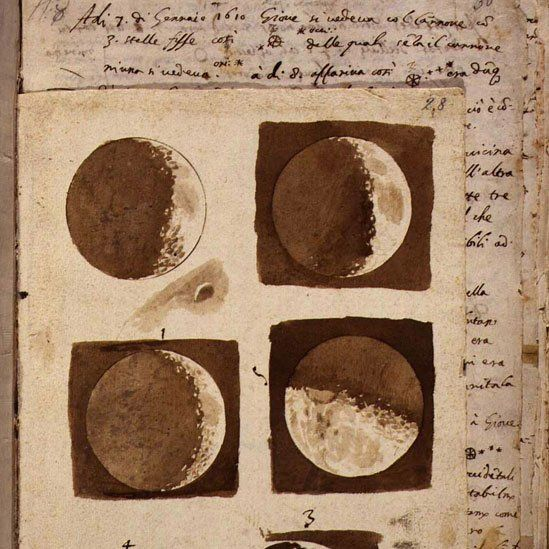
\includegraphics[width=0.6\textwidth]{images/ilustracion_galileo.jpg}
	\caption{Ilustración de la Luna hecha por Galileo Galilei en 1610. Presentada en su obra Siderus Nuncius.}
	\label{fig:ilustracion_luna_galileo_1610}
\end{figure}

Con el tiempo, se empezó a investigar el uso de espejos para captar luz, en lugar de lentes. Esto permitía evitar problemas comunes en los telescopios con lentes. En 1668, Isaac Newton construyó el primer telescopio reflector funcional, conocido hoy como Telescopio Reflector Newtoniano (\ref{fig:telescopio_reflector_newotoniano}). Este invento ocupa un espejo cóncavo, de una aleación de cobre y estaño pulido, en lugar de lentes para magnificar una región del espacio evitando aberraciones cromáticas. 

 
%\begin{table}[h!]
%\centering
%\caption{Tabla comparativa de telescopios refractarios vs reflectores}
%\begin{tabular}{ |p{3cm}||p{3cm}|p{3cm}|p{3cm}|  }
%	\hline
%	\multicolumn{4}{|c|}{Telescopes comparison} \\
%	\hline
%	 & Refractor & Reflector & Mezcla \\
%	\hline
%	Materiales & AF    &AFG&   004\\
%	Ventajas&   AX  & ALA   &248\\
%	Fabricación &AL & ALB&  008\\
%	Limitantes &DZ & DZA&  012\\
%	\hline
%\end{tabular}
%\end{table}
% SUGERENCIA: incluir una tabla comparativa simple: refractor vs reflector (material, ventajas, época).
% O una ilustración estilo línea de tiempo con telescopios clave.

Durante más de un siglo, los telescopios refractores evolucionaron lentamente, hasta que en 1730 se desarrollaron lentes acromáticas, lo que mejoró significativamente la calidad de imagen. Por otro lado, los primeros telescopios reflectores enfrentaban un problema relacionado con la pérdida de brillo en los espejos metálicos (fig \ref{fig:espejo_metalico_especulum}). Este problema se fue solucionado progresivamente en la década de 1850 con la introducción de espejos de vidrio recubiertos, y más adelante, en 1932, con la implementación de espejos aluminizados.

%\begin{figure}[H]
%	\centering
%	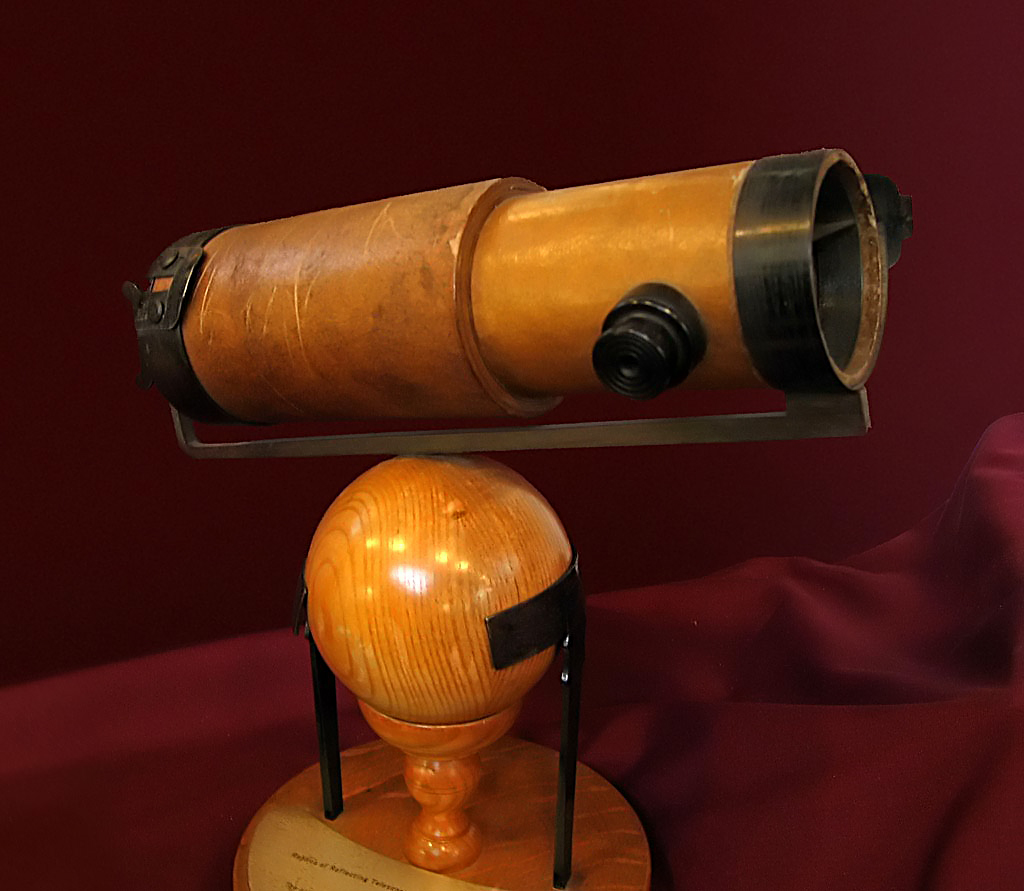
\includegraphics[width=0.6\textwidth]{newton_reflector_telescopio.jpg}
%	\caption{Réplica del primer telescopio reflector registrado por Isaac Newton ante la Royal Society en 1672.}
%	\label{fig:telescopio_reflector_newotoniano}
%	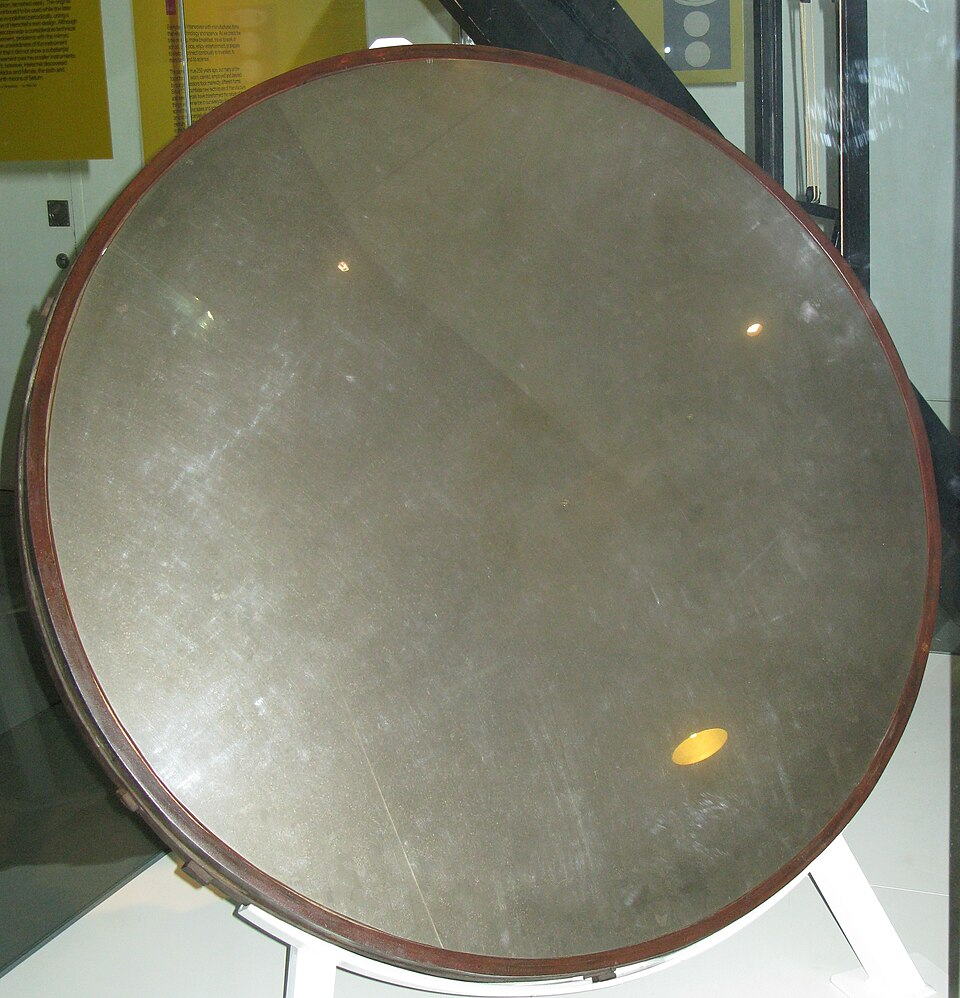
\includegraphics[width=0.6\textwidth]{speculum_mirror_metal.jpg}
%	\caption{Espejo metálico de 1.2m de diámetro para un telescopio de 40pies.}
%	\label{fig:espejo_metalico_especulum}
%\end{figure}

En aquella época, los telescopios refractores más grandes alcanzaban aperturas de aproximadamente $1\,\mathrm{m} \approx 39\,\mathrm{in}$, mientras que los reflectores superaban los $10\,\mathrm{m} \approx 33\,\mathrm{ft}$. Actualmente, se están construyendo telescopios aún más grandes, con aperturas entre $30$ y $40\,\mathrm{m}$, telescopios que se ubican en órbita para evitar interferencias con la atmósfera. Sin embargo, la utilización de telescopios ópticos terrestres continúa siendo de gran interés científico debido a las nuevas tecnologías las cuales ofrecen soluciones adaptativas, de bajo costo y gran impacto en investigación. Además de los nuevos algoritmos de procesamiento de imágenes y de corrección de aberraciones ofrecen un gran marco teórico para el desarrollo de instrumentos ópticos (fig \ref{fig:gran_telescopio_canarias} \ref{fig:gmt_chile}). 

\begin{figure}[H]
	\centering
	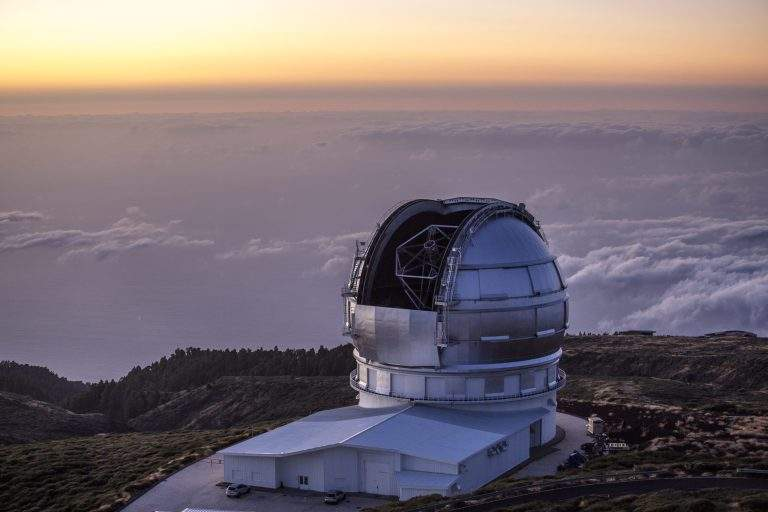
\includegraphics[width=0.6\textwidth]{gran_telescopio_canarias.jpg}
	\caption{Gran telescopio de Canarias (GTC). Telescopio reflector con 10.4m de diámetro de espejo principal, compuesto por 36 segmentos hexagonales.}
	\label{fig:gran_telescopio_canarias}
	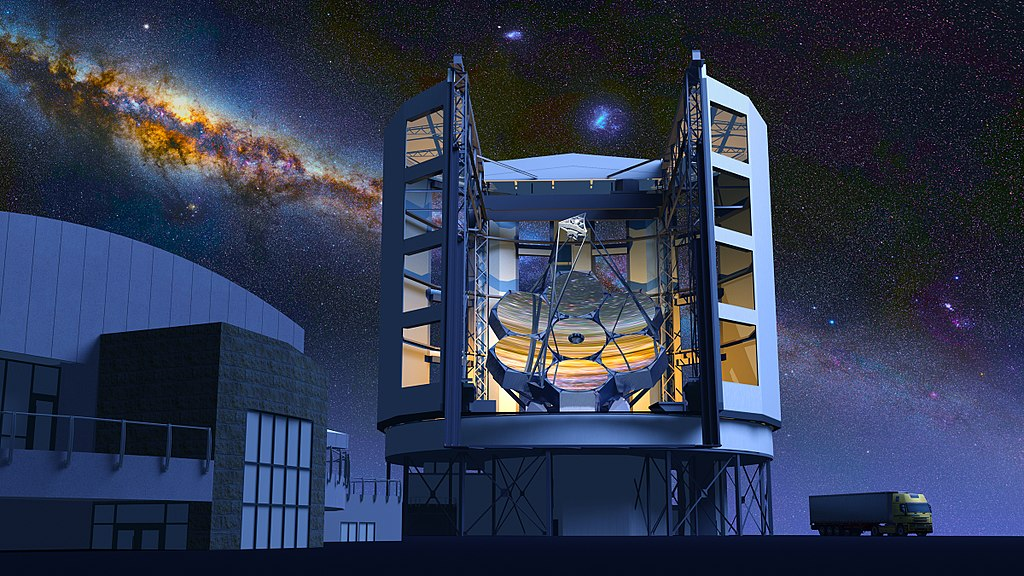
\includegraphics[width=0.6\textwidth]{giant_magallan_telescope.jpg}
	\caption{Giant Magellan Telescope (GMT) es uno de los tres proyectos de telescopios más grandes actualmente en construcción, en el desierto de Atacama - Chile.}
	\label{fig:gmt_chile}
\end{figure}


 
% SUGERENCIA: 
% insertar una animación con transición de escalas.


\section{Principios Ópticos Fundamentales}
\subsection*{La luz y su velocidad}

La luz, tal como la percibimos, corresponde a una fracción del espectro electromagnético la cual puede ser detectada por nuestro sistema visual. Su definición, en términos prácticos, está íntimamente relacionada con la respuesta fisiológica y psicológica del sistema ojo-cerebro frente a estímulos dentro del rango de la luz visible, que abarca frecuencias entre $400$ y $700 nm$.

Por ejemplo, una mezcla de luz roja y verde es interpretada por nuestro sistema visual como luz amarilla, aunque no exista radiación electromagnética en la longitud de onda correspondiente al amarillo. Este fenómeno se conoce como \textit{mezcla aditiva de colores} y es una propiedad emergente de cómo procesamos la luz, más que de la luz en sí misma.

\vspace{0.3cm}
% FIGURA sugerida: diagrama con el espectro visible y un círculo de mezcla RGB

%\subsection{Breve historia de la medición de la velocidad de la luz}

Desde hace siglos, el ser humano ha intentado determinar si la luz tiene velocidad finita o es instantánea. Con el desarrollo de los telescopios, comenzaron a surgir los primeros experimentos.

%\subsubsection{Intento de Galileo}

Galileo Galilei, en el siglo XVII, intentó medir la velocidad de la luz con la ayuda de un asistente. Cada uno portaba una linterna, y se situaban a unos 3 kilómetros de distancia. Galileo destapaba su linterna, y cuando su asistente veía la luz, destapaba la suya en respuesta. Galileo cronometraba el tiempo entre su acción inicial y la recepción de la segunda luz.

Aunque ingenioso, el experimento no tuvo éxito. Hoy sabemos que la luz recorre 3 kilómetros en aproximadamente $10^{-5}$ segundos, un tiempo imposible de medir con instrumentos de la época, además no se consideraba el factor de error humano.


\vspace{0.3cm}
% ILUSTRACIÓN sugerida: recreación simple del experimento con linternas

%\subsubsection{Ole Rømer y las lunas de Júpiter}

En 1675, el astrónomo danés Ole Rømer estudió durante varios años los eclipses de la luna Io, una de los satélites naturales de Júpiter. Rømer, observó que la duración entre eclipses variaba dependiendo de la posición relativa entre la Tierra y Júpiter. Cuando la Tierra se alejaba de Júpiter, los eclipses parecían retrasarse.

Rømer concluyó correctamente que la luz tardaba un tiempo finito en viajar, y que esta diferencia se debía al cambio en la distancia. Su trabajo fue el primer indicio experimental de que la luz no tenía velocidad infinita.

\vspace{0.3cm}
% ILUSTRACIÓN sugerida: esquema Tierra-Júpiter con Io mostrando trayectos de luz más largos/cortos

% \subsection{James Bradley}

Por otro lado, James Bradley, un físico de Inglaterra con la ayuda de telescopios descubre un cambio simétrico (paralaje), es decir, observó el desplazamiento cíclico de toda la esfera celeste a lo largo del año, con un pico máximo de cambio, lo que ocurría con la tierra con una velocidad orbital dada, lo que se explicaba con el movimiento de la tierra alrededor del sol, respaldando la teoría heliocentrista, y por una velocidad finita de la luz. Estimó $\sim 301,000 km/s$.



%\subsubsection{Método de Fizeau (1849)}

% En 1849, el físico francés Hippolyte Fizeau diseñó un ingenioso experimento para medir la velocidad de la luz en laboratorio. Utilizó una rueda dentada giratoria y un haz de luz que atravesaba uno de los espacios entre los dientes hacia un espejo situado a unos 8 km de distancia. El haz se reflejaba y regresaba a través de la misma rueda.

% Cuando la rueda giraba a una velocidad específica, el haz reflejado era bloqueado por el siguiente diente. Midiendo esa velocidad de rotación y la distancia al espejo, Fizeau logró estimar el tiempo de viaje de la luz y, con ello, su velocidad.

% Este fue el primer experimento exitoso para medir la velocidad de la luz sin necesidad de observaciones astronómicas.

\vspace{0.3cm}
% FIGURA sugerida: diagrama de la rueda dentada, fuente de luz, espejo a distancia

%\subsubsection{Método de Michelson (1879)}

% Albert A. Michelson, en 1879, perfeccionó el método de Fizeau. En lugar de una rueda dentada, utilizó un espejo giratorio de alta precisión. El haz de luz se reflejaba hacia un espejo fijo a varios kilómetros, y luego regresaba.

% Durante ese tiempo, el espejo giratorio cambiaba de orientación, lo que hacía que el haz de retorno se desviara. Midiendo con precisión ese ángulo de desviación, Michelson pudo calcular con mayor exactitud el tiempo de viaje de la luz y, por lo tanto, su velocidad.

% Este método se convirtió en uno de los más confiables del siglo XIX, y Michelson fue reconocido con el Premio Nobel en 1907, siendo el primer estadounidense en recibirlo por un trabajo de física.

\vspace{0.3cm}
% FIGURA sugerida: diagrama del espejo giratorio y trayectoria desviada del haz

%\subsection{Relación con las constantes electromagnéticas}

Hoy en día, uno de los métodos más exactos para conocer la velocidad de la luz es a través de las constantes del electromagnetismo. La relación fundamental es:

\[
c = \frac{1}{\sqrt{\epsilon_0 \mu_0}}
\]

Donde:
\begin{itemize}
	\item $\epsilon_0$ es la permitividad eléctrica del vacío ($8.854 \times 10^{-12}\, \text{F/m}$),
	\item $\mu_0$ es la permeabilidad magnética del vacío ($4\pi \times 10^{-7}\, \text{N/A}^2$).
\end{itemize}

Esta ecuación, derivada de las ecuaciones de Maxwell, describe cómo los campos eléctricos y magnéticos se propagan en el vacío. A partir de estas constantes, se puede demostrar que la velocidad de propagación de cualquier onda electromagnética en el vacío es constante y finita, por lo tanto siendo la luz una perturbación del campo electromagnético, la velocidad de la luz en el vacío es constante y finita: 
(añadir anexos con los calculos para esto)

\begin{mybox}[blue]{Velocidad de la luz en el vacío}[colbacktitle=blue!30!white, coltitle=black]
	$c = 299\,792\,458 \, \text{m/s} \approx 3\cdot10^8 \text{m/s}$ 
\end{mybox}



\vspace{0.3cm}
% FIGURA sugerida: resumen visual con ecuación, valor de c, y conexión con unidades SI

%\begin{mybox}[green]{Espacio Vectorial}[colbacktitle=blue!30!white, coltitle=black]
%	Un conjunto con dos operaciones (suma y producto por escalar) que satisfacen 8 axiomas.
%\end{mybox}
%
%\begin{mybox}[gray]{Espacio Vectorial}[colbacktitle=blue!30!white, coltitle=black]
%	Un conjunto con dos operaciones (suma y producto por escalar) que satisfacen 8 axiomas.
%\end{mybox}

\section*{Propagación de la luz}

La propagación de la luz, al tratarse de una oscilación del campo electromagnético, está regida por la ecuación de onda. No obstante, mucho antes de que Maxwell desarrollara la teoría del electromagnetismo, la propagación de la luz ya había sido descrita empíricamente mediante dos principios fundamentales: el \textbf{Principio de Huygens} y \textbf{el Principio de Fermat}.

El principio de Huygens, propuesto por el físico holandés Christiaan Huygens en el siglo XVII, describe el comportamiento de los frentes de onda de forma geométrica:

\begin{mybox}[green]{Principio de Huygens}[colbacktitle=blue!30!white, coltitle=black]
	Cada punto de un frente de onda primario actúa como foco, o fuente, de ondas esféricas secundarias que se propagan con la misma velocidad y frecuencia que la onda original. El nuevo frente de onda, al cabo de un intervalo de tiempo, es la envolvente de estas ondas secundarias.
\end{mybox}

Por otro lado, el principio de Fermat, basado en una idea geométrica y variacional, establece:

\begin{mybox}[green]{Principio de Fermat}[colbacktitle=blue!30!white, coltitle=black]
	La trayectoria que sigue la luz al pasar de un punto \textbf{A} a un punto \textbf{B} es aquella en la que el tiempo de recorrido es mínimo. Es decir, la luz tiende a seguir el camino óptico más rápido.
\end{mybox}

\vspace{0.3cm}
% FIGURA SUGERIDA: Comparación visual de Huygens y Fermat con una superficie separadora aire-vidrio

Estos principios no solo son compatibles, sino que se complementan. El primero ofrece una visión geométrica local, útil para explicar fenómenos como la difracción, mientras que el segundo permite deducir leyes globales como la de la refracción.

\section{Reflexión y Refracción}

La velocidad de la luz en medios transparentes como el aire, el agua o el vidrio es menor que su velocidad en el vacío. Esta diferencia da lugar a un parámetro óptico llamado \textbf{índice de refracción}, este está definido como:

\begin{mybox}[blue]{Índice de refracción}[colbacktitle=blue!30!white, coltitle=black]
	$n = \frac{c}{v}$
\end{mybox}

donde:
\begin{itemize}
	\item $c$ es la velocidad de la luz en el vacío,
	\item $v$ es la velocidad de la luz en el medio considerado.
\end{itemize}

Cuando un rayo de luz incide sobre la interfaz entre dos medios con diferente índice de refracción (por ejemplo, aire y vidrio), una parte de la energía se refleja y otra parte penetra en el segundo medio, cambiando de dirección: este fenómeno se conoce como \textbf{refracción}.

% FIGURA: ya está incluida: refraction_reflection.png

\begin{figure}[H]		
	\centering
	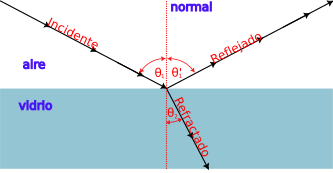
\includegraphics[width=0.6\textwidth]{images/refraction_reflection.png}
	\caption{El ángulo de reflexión es igual al ángulo de incidencia. El ángulo de refracción $\theta_2$ depende de la relación entre las velocidades de propagación en ambos medios.}
	\label{fig:refraccón_reflexión_planos}
\end{figure} 

En la figura \ref{fig:refraccón_reflexión_planos} se observa un rayo de luz incidente sobre la superficie de un vidrio. El ángulo $\theta_1$ entre el rayo incidente y la normal se denomina \textbf{ángulo de incidencia}, y el plano definido por ambos se llama \textbf{plano de incidencia}.

El rayo reflejado se encuentra en el mismo plano y forma un ángulo igual con la normal, lo cual se expresa con la \textbf{ley de la reflexión}:

\begin{mybox}[blue]{Ley de la reflexión}[colbacktitle=blue!30!white, coltitle=black]
	$\theta'_1 = \theta_1$
\end{mybox}

Por otro lado, el rayo que entra al segundo medio (el rayo \textbf{refractado}) cambia de dirección debido al cambio de velocidad de propagación. La relación entre los ángulos y las velocidades en cada medio se expresa como:

\begin{equation}
	\frac{1}{v_1} \sin(\theta_1) = \frac{1}{v_2} \sin(\theta_2)
	\label{eq:refraccion_dos_medios}
\end{equation}

Si sustituimos las velocidades por sus respectivas expresiones en términos del índice de refracción ($v = c/n$), obtenemos la conocida \textbf{ley de Snell}:

\begin{mybox}[blue]{Ley de Snell de la refracción}[colbacktitle=blue!30!white, coltitle=black]
	$n_1 \sin(\theta_1) = n_2 \sin(\theta_2)$
\end{mybox} 

\vspace{0.3cm}
% FIGURA sugerida extra (opcional): simulación de cómo cambia el ángulo de refracción con diferentes índices

\subsection{Mecanismos físicos de la reflexión y la refracción}

A nivel microscópico, la reflexión y la refracción pueden entenderse como fenómenos de interacción entre la luz y los átomos del medio. Cuando un rayo de luz incide sobre una superficie, sus campos eléctricos hacen oscilar las cargas (principalmente electrones) en los átomos del material. Estas oscilaciones inducidas producen una nueva radiación: la luz es absorbida y reemitida por los átomos.

En el fenómeno de la reflexión, parte de las ondas reemitidas se propagan en dirección opuesta al haz de luz incidente. Debido a interferencias constructivas (coherencia de la onda incidente) estas ondas se reflejan constructivamente en una dirección bien definida, formando el rayo reflejado. 

En el caso de la refracción, la luz reemitida hacia adelante también sufre interferencia constructiva, pero en una dirección distinta a la original. El resultado neto es un cambio en la dirección de propagación, determinado por la diferencia de velocidades de fase en cada medio.



% NOTA: esta explicación es un paso hacia modelos electromagnéticos, pero aún accesible a estudiantes de primeros semestres

\subsection*{Reflexión Especular y Difusa}

La reflexión especular ocurre en superficies suaves y lisas. Podemos observar en la imagen \ref{fig:ref_especular_difusa} donde los rayos de luz del objeto $P$ al reflejar en el espejo forman una imagen como si procediecen del punto $P'$, este se denomina \textbf{imagen virtual del punto $P$}.
Por otro lado, la reflexión difusa ocurre cuando la superficie donde se refleja la imagen es rugisa, es decir, los rayos procedentes de un puesto se reflejan en todas direcciones y no divergen de ningún punto. 

\begin{figure}[H]
	\centering
	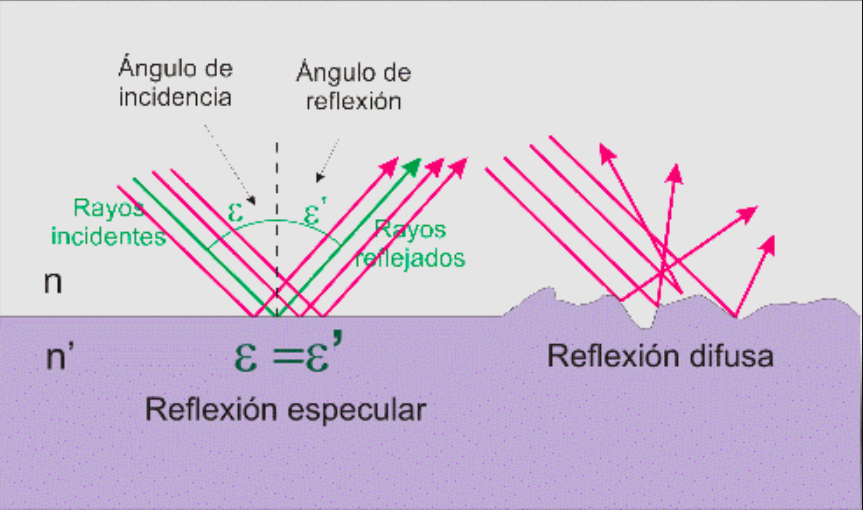
\includegraphics[width=0.6\textheight]{ref_especular_difusa.png}
	\caption{Reflexion especular y difusa.}
	\label{fig:ref_especular_difusa}
\end{figure}

% Intensidad de relativa de la luz reflejada y transmitida
% Reflexión interna total
%% Fibra óptica
% Espejismo

\subsection*{Dispersión}

El índice de refracción de un material depende ligeramente de la longitud de onda con la que incide un haz de luz. Para la mayoría de materiales, $n$ disminuye cuando crece la longitud de onda. La dependencia entre el índice de refracción con la longitud de onda (y por tanto con la frecuencia) se denomina \textbf{dispersión}.

\begin{figure}[H]
	\centering
	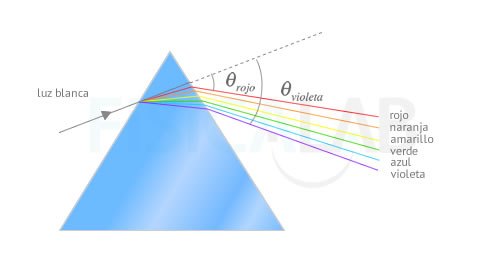
\includegraphics[width=0.6\textwidth]{images/descomposicion_luz.jpg}
	\caption{Imagen de la descomposición de la luz blanca cuando atraviesa un prisma.}
	\ref{fig:dispersion_prisma_luz}
\end{figure}

% Arcoiris.

% Polarización
%% Polarización por absorción
%% Polarización por reflexión
%% Polarización por dispersión(o scattering)
%% Polarización por birrefringencia


% Dualidad Onda- Partícula
% Espectros de Luz
% Fuentes luminosas, líneas espectrales

\subsection{Reflexión y espejos}

\subsubsection*{Espejos Planos}
Los espejos planos, los más conocidos. Podemos observar la figura \ref{fig:espejos_planos}, en ella se ilustran dos rayos que se emiten de los extremos de la botella (en realidad van en todas las direcciones), estos son los que encierra el haz de rayos de luz que entra al ojo. Cada conjunto de rayos divergentes que se reflejan en el espejo y entran en el ojo parecen provenir de un mismo punto (llamado punto de imagen) detras del espejo, tal y como muestran las líneas punteadas. Siempre que un objeto esté dentro del plano de un espejo existe una posición en la cual puede situarase el ojo para poder ver la imagen. 

\begin{figure}[H]
	\centering
	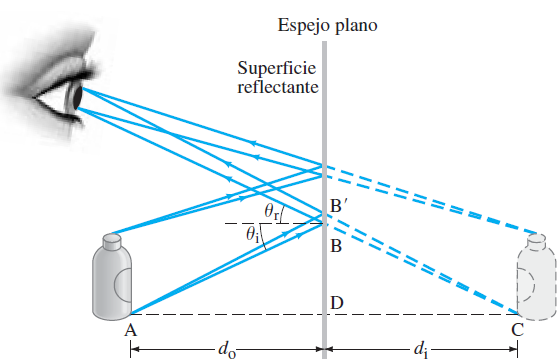
\includegraphics[width=0.6\textwidth]{images/espejo_plano.png}
	\caption{Espejo plano reflejando una botella. Se marcan los puntos que son los que entrarán al ojo.}
	\label{fig:esplejos_planos}
\end{figure}

En los espejos también podemos observar el resultado de inversión en profundidad, es decir, si ponemos la mano derecha en el espejo vemos convertida en la mano izquierda, también podemos observarlo como un cambio de coordenadas, donde el espejo transforma un sistema de coordenadas según la regla de la mano derecha, donde $\hat{i} \times \hat{j} = \hat{k}$ se convierte en $\hat{i} \times \hat{j} = -\hat{k}$. 

\begin{figure}[H]
	\centering
	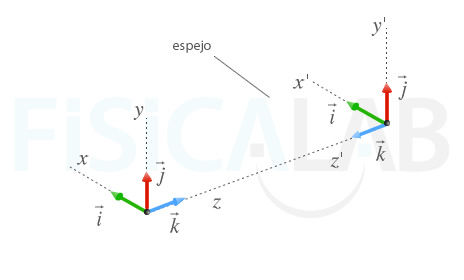
\includegraphics[width=0.6\textwidth]{images/inversion_profundidad.jpg}
	\caption{.}
	\label{fig:inversion_profundidad}
\end{figure}

\subsubsection*{Espejos Esféricos}

Podemos observar la figura \ref{fig:espejo_esferico}, que muestra un haz de rayos que provienen del punto $P$ situado en el eje de un espejo esférico cóncavo y  que después de reflejarse en él convergen en el punto $P'$, también denominado \textbf{imagen real}. Se le denomina imagen real porque la luz realmente emana del punto imagen, esta puede ser vista por cualquier observador al lado izquierdo del espejo. (Regresar a la explicación de imagenes virtuales en espejos planos). 

\begin{figure}[H]
	\centering
	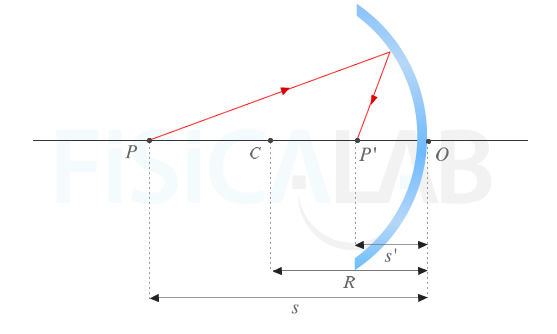
\includegraphics[width=0.6\textwidth]{images/espejo_esferico_AV.jpg}
	\caption{Los rayos procedientes del punto $P$, en el eje $PO$ de un espejo esférico concavo forman una imagen en $P'$. Los rayos más significativos son los que inciden más cercanos al eje $PO$.}
	\label{fig:espejo_esferico}
\end{figure}

En los espejos cóncavos también se pueden generar aberraciones denominadas \textbf{aberraciones esféricas}. Los rayos que rebotan más lejanos al eje $PO$ son los causantes de estas aberraciones, esto es debido a que estos rayos no consiguen pasar exactamente por el punto de la imagen.

Para cálculos relacionados a espejos esféricos queremos buscar una ecuación que relacione el punto $P$ con el punto $P'$. 

\begin{figure}[H]
	\centering
	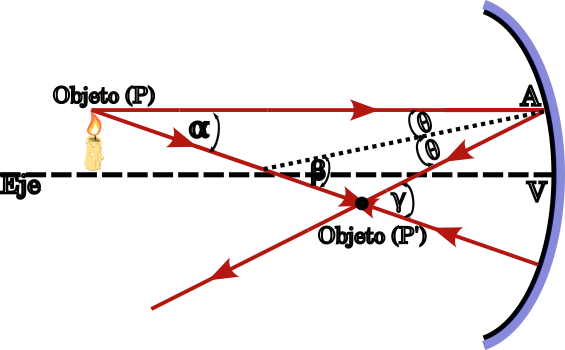
\includegraphics[width=0.6\textwidth]{images/geometria_espejos.png}
	\caption{Geometría para espejos}
	\label{fig:geometria_espejos_imagen}
\end{figure}

Siguiendo identidades trigonométricas, se llega a la conclusión de que 
\begin{equation}
	\alpha + \gamma = 2\beta
\end{equation}

\subsubsection{Fabricación Espejos}


\subsection{Refracción y Lentes}
%Para crear lentes se pulen cilindros de vidrio para formar superficies esféricas convexas. Suponiendo que todos los rayos son paraxiales, mediante la aproximación de ángulos pequeños tenemos $\alpha \approx l/s$, $\beta = \approx l/r$, $\gamma = l/s'$. 
%
%\begin{equation}
%	\frac{1}{s} + \frac{1}{s'} = \frac{2}{r}
%\end{equation}

Todos estamos familiarizados con el fenómeno de ver cambiar la dirección de la luz que proviene de un objeto cuando la mitad del mismo está sumergido en un medio distinto al aire, como el agua. Este fenómeno, de "doblamiento" de la luz al pasar de un medio a otro, es lo que se denomina refracción. 

Este fenómeno ocurre porque la velocidad de la luz cambia al pasar de un medio a otro. Como sabemos, la luz viaja a su máxima velocidad en el vacío, cuando entra a un medio distinto, su velocidad se ve reducida. 

Para cuantificar esta disminución de velocidad en el medio, utilizmaos el índice de refracción $n$. El índice de refracción de un medio se define como la relación entre la velocidad de la luz en el vacío y la velocidad de la luz en ese medio.

\begin{equation}
	n = \frac{c}{v}
	\label{eq:indice_refraccion}
\end{equation}

Cada material tiene su propio indice de refracción, por ejemplo, el indice de refracción del aire es 1.003, el del agua 1.33, y del vidrio es 1.5. Cuanto mayor sea el índice de refracción, más ltena es la luz que viaja en ese medio. 

Para entender como la luz cambia de dirección al refractarse ocupamos la \textbf{ley de Snell}¨. Esta ley relaciona los ángulos de incidencia y refracción con los índices de regracción de los dos medios en el punto de separación. 

\begin{figure}[ht]
	\centering
	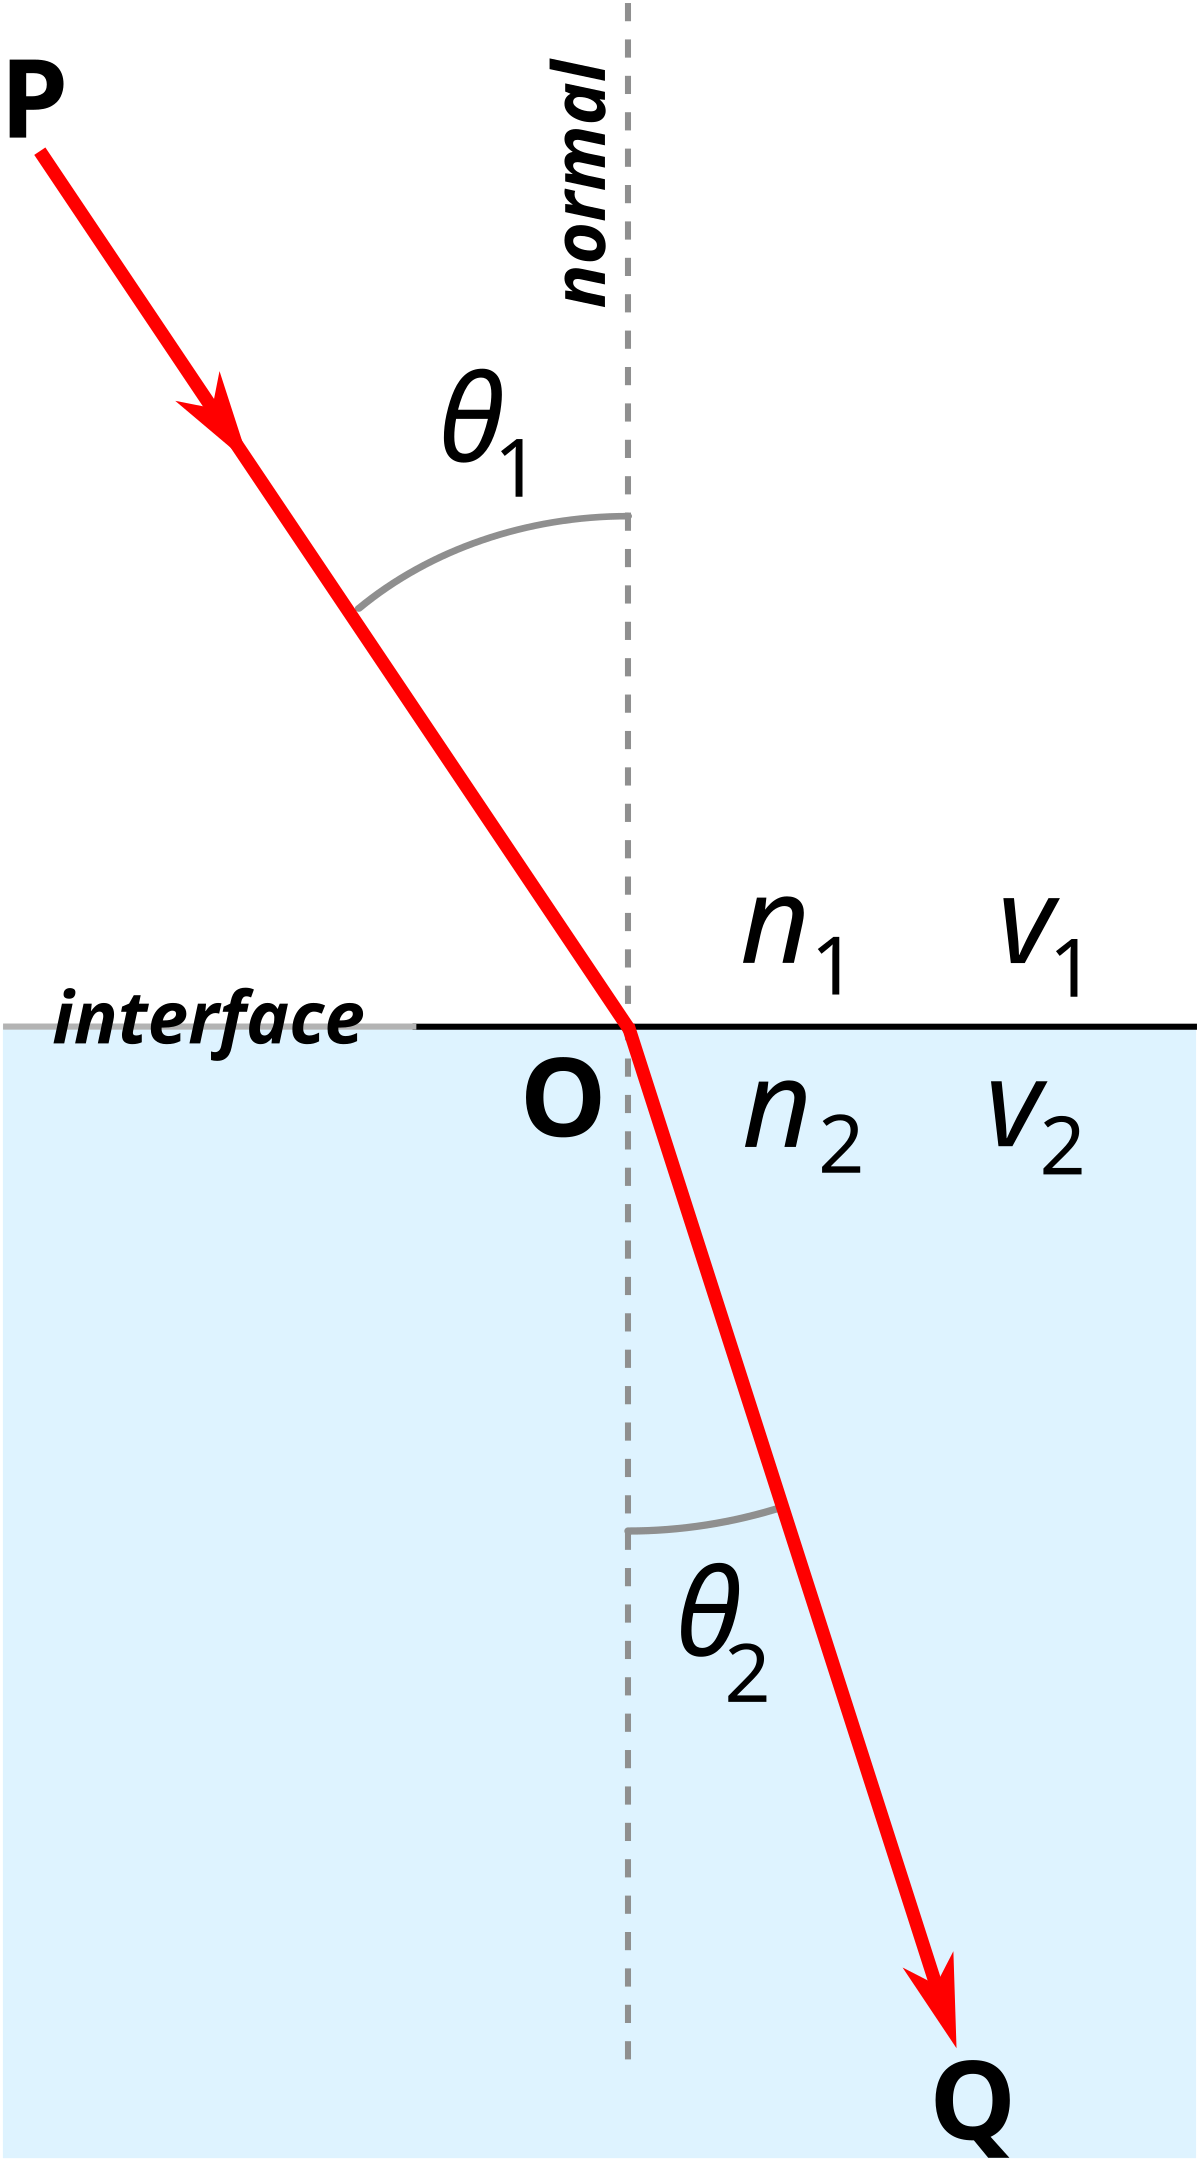
\includegraphics[width=0.5\textwidth]{images/Snells_law2.png}
	\caption{Se puede observar la interacción entre un rayo de luz que incide una superficie que separa dos medios. Observamos el ángulo de incidencia $a$, es el ángulo entre el rayo incidente y la línea \textbf{normal}, una línea perpendicular a la superficie en el punto de incidencia. }
	\label{fig:snell_law}
\end{figure}

Cuando la luz pasa de un medio con índice de refracción menor a uno con índice de refracción mayor $n1 < n2$, el haz de luz se acerca a la normal $r<i$, esto pasa por ejemplo cuando del aire pasa al agua o al vidrio. 

Contrario a esto, cuando la luz pasa de un medio $n1 > n2$ la luz se aleja de la normal $r > i$, esto ocurre cuando la luz pasa del agua al vidrio o aire.

Con respecto al comportamiento ondulatorio de la luz puede entenderse con la entrada en un medio donde su velocidad es diferente, una parte del frente de onda se relentiza o acelera antes que la otra, lo que provoca que el frente de onda cambie de dirección. 

En un principio, Fermat fue quien proporcionó una idea fundamental en la refracción de la luz, estableciendo que ella sigue el camino que le toma menor tiempo para viajar entre dos puntos. Cuando la luz pasa de un punto A a un punto B entre dos medios con distinta velocidad, este va a seguir la trayectoria que minimiza el tiempo de viaje. 

Considernado el índice de refracción, el tiempo que tarda en recorrer una distancia $d$ en un medio con indice de refracción $n_1$ es proporcional a $nd$. La cantidad $nd$ se conoce como \textbf{camino óptico}.

Un fenómeno óptico con respecto a este principio es la \textbf{refracción total interna}, se puede observar cuando la luz viaja de un medio con indice de refracción mayor hacia uno coon uno con índice de refracción menor y esta incide con un ángulo bastante grande, el haz de luz no se refracta hacia el segundo medio, sino que se refleja completamente en el interfaz. 

% EJEMPLO AGUA CON AZUCAR MUY SATURADA

Por otro lado, los lentes, son dispositivos ópticos limitados por dos superficies refringentes (dioptrios), donde al menos una de ellas es esférica. Existen distintos tipos de lentes para telescopios, y dependiendo de esta la luz se refracta al entrar y salir en distinta forma. Las lentes convergentes, o también denominadas convexas, son más anchas en el centro y más delgadas en los bordes. Cuando los rayoso de luz paralelos, haciendo una aproximación a infinito, con la posición de los astros. 

% REFRACCION

Las lentes convergentes, o también conocidas como convexas, son más anchas por el centro y más delgadas en los bordes. Cuando rayos de luz paralelos inciden sobre una lente convergente se refractan y convergen en un punto llamado el \textbf{punto focal o foco}. Los telescopios refractores utilizan estos lentes convergentes como objetivo para recolectar y enfocar la luz de objetos distantes. Una lupa es un ejemplo de lente convergente, si un objeto está muy lejos, una lente convergente forma una imagen real e invertida acerca de su punto focal. 

Lentes divergentes, también conocidas como cóncavas, son más delgadas en el centro y más anchas en los bordes. Cuando rayos paralelos de luz inciden sobre una lente divergente se refractan y divergen, es decir, se separan. Las lentes divergentes forman una imagen virtual, derecha más pequeña que el objeto real. En telescopios refractores se utiliza una lente divergente como ocular para el diseño galileano. 

En un telescopio refractor, la lente principal recoge la luz del objeto celeste y la refracta hasta concentrarse en su foco, donde otra lente, el ocular se encarga de aumentar el tamaño angular aparente de la imagen. 

\subsubsection{Fabricación de lentes}

La fabricación de lentes implica talalr y pulir piezas de vidrio, generalmetne de forma esférica. Para las lentes acromáticas, se requiere un proceso de unión precisas (cimentación) de los dos o más elementos del vidrio con diferentes índices de refracción y dispersión. Los parámetros de diseño de la lente, incluyendo el radio de curvatura, el grosor central y otros, se calculan meticulosamente para garantizar un rendimiento óptico óptimo. Los materiales comunes para las lentes acromáticas positivas y negativas son el vidrio \textbf{N-BK7} (para la corona) y \textbf{SF5} (pedernal). Para las lente triplete acromáticas, se puede utilizar vidrio óptico tradicional, slice fundida (diferentes grados) y fluoruro de calcio (CaF2), entre otros. La precisión en la fabricación es crucial para obtener la forma correcta de las superficies y asegurar la correcta alineación de los elementos en las lentes compuestas. 

\subsection{Combinación Lentes-Espejos}

Existen sistemas de combinaciones entre lentes-espejos, para distintos tipos de instrumentos ópticos como cámaras o telescopios. Estos utilizan estas combinaciones de elementos ópticos para captar o mejorar la forma en la que se obtiene la luz de algún objetivo. 

% Agregar más informacion, pedirle a gpt.


\section{Tipos de Telescopios}
% Tipos y características
Como se mencionó al incio, la palabra \textbf{telescopio} hace referencia a una serie de instrumentos, no sólo el telescopio óptico, pese a que se ha generado gran confusión con respecto a su uso. Al final, la etimología lleva a entender que se busca "ver a lo lejos", pero va más allá de ver con los ojos. Los telescopios también abarcan zonas del espectro que pertenecen al espectro electromagnético pero están mucho más allá del rango de la frecuencia de la luz visible. 

Existen radiotelescopios, especializados en escuchar el espacio

También existen telescopios en el rango de infrarrojo o ultravioleta, cada uno especializado en observar una región del universo en una frecuencia con algún objetivo. 



\subsection{Telescopios Refractores}


En los telescopios refractores, la lente objetivo (convergente) en la parte frontal del tubo recoge la luz del objeto celeste y la refracta hasta concentrarse en su foco, donde se forma una imagen real. Luego, el ocular puede ser otra lente convergente (en diseños modernos) o una lente divergente (en el diseño galileano), esta se utiliza para aumentar el tamaño angular aparente de la imagen, permitiendo que el observador vea una imagen ampliada del objeto distante.

En este tipo de telescopios es necesario tomar en cuenta la \textbf{distancia focal}, la cual es la distancia entre la lente objetivo y el punto donde los rayos paralelos convergen (o parecen divergir). La longitud del tubo del telescopio refractor es aproximadamente la suma de la distancia del objetivo y la distancia focal del ocular (Revisar \ref{subsec:dist_focal}¨ 

El aumento total del telescopio se define como la razón entre la altura de la imagen y la altura del objeto, o la razón entre la longitud focal del objetivo y la longitud focal del ocular. (Revisar \ref{subse:aumento_resolucion})

Existen una serie de problemas relevantes con los telescopios refractores, es la \textbf{aberración cromática}, y la \textbf{aberración esférica}. Isaac Newton descubrió que la luz blanca estaba compuesta por diferentes colores, y cuando la luz blanca atraviesa un prisma (una lente que actua como prisma), cada color se desvía o refracta en un ángulo ligeramente diferente. Los rayos periféricos que ingresan por el objetivo de un telescopio refractor no llegan a concentrarse en el mismo punto focal, lo que causa que el borde del objeto no sea nítido y presente colores. Esto es causado porque el índice de refracción de un material varía un poco con la longit de onda de la luz. 

Por otro lado, la aberración esférica es causada por la curvatura esférica de las lentes, que hace que rayos que pasan por diferentes partes de la lente se enfoquen en focos ligeramente distintos, resultando en una imagen borrosa. 

Para minimizar las aberraciones los telescopios actuales utilizan una serie de objetivos compuestos por uno o varias lentes. Un avance significativo es el desarrollo de las \textbf{lentes acromáticas}. Este tipo de lentes son específicamente diseñadas para limitar los efectos de la aberración cromática y esférica. Generalemente se fabrican de forma que permiten enfocar dos longitudes de onda de luz en un mismo punto (generalmente roja y azul), reduciendo así su aberración cromática. 

Estas lentes generalmente están fabricadas de vidrio con propiedades ópticas específicas, específicamente se realizan de una mezcla de vidrio de pedernal (alta dispersión de luz) con corona de cristal (baja dispersión de luz), estos dos elementos se cementan entre sí para formar un lente doble y debido a esta combinación de materiales se puede contrarestar la dispersión de luz.

Cuando la luz entra en la lente de \textbf{corona de cristal}, se refracta, pero las diferentes longitudes de onda aún se enfocan en puntos ligeramente diferentes debido a su baja dispersión. Luego la luz pasa a través de la lente de \textbf{vidrio de pedernal}, que tiene una mayor dispersión y desvía más la luz. La curvatura negativa de la lente de cristal de pedernal contrarresta la curvatura postivia de la lente de cristal de corona, asegurando que dos longitudes de onda, la roza y azúl converjan en un mismo punto focal, reduciendo mucho la aberración cromática y dando como resultado una imagen más clada.

Existen dos tipos de lentes acromáticas, 

Lentes acromáticas positivas: Suelen ser un doblete con un elemento positivo de bajo índice de refracción (vidrio de la corona) y un elemento negativo de alto índice de refracción (vidrio de pedernal).

Lentes acromáticas negativas: utilizan combinaciones similares de materiales

Lentes triplete acromáticas: compuestas de tres elementos de lente, típicamente dos de alto índice de refracción y uno de menor índice de refracción en el medio. ESte diseño reduce aún más las aberraciones, incluyendo la distorsión y aberración esférica. 

Lentes acromáticas asféricas, combinan una lente acromática con una lente asférica para mitigar los errores del frente de onda y reducir la aberración esférica, ofreciendo una mejor calidad de imagen. 



\subsection{Telescopios Reflectores}

El origen de los telescopios reflectores está por el lejano 1668, donde Isaac Newton construyó su propia versión de un telescopio que utilizaba espejos en lugar de lentes. Esta idea surgió de su descubrimiento de que la luz blanca se descompone en distintos colores al pasar aa través de un prisma y que la lente actúa como una especie de prisma. Newton observó que un espejo curvado enfoca la luz de la misma manera que un lente, pero la luz rebota en la superficie del espejo y no la atraviesa, eliminando así la dispersión de colores. 

El primer telescopio reflector de Newton tenía apenas 15.5 cm de longitud y utilizaba un espejo curvo de menos de 4cm de diámetro en la base del tubo. La luz entraba y se reflejaba en este espejo curvo, luego en un espejo plano y terminaba enfocándose en un ocular. Este pequeño telescopio tuvo funcionalidades similares a un refractor de 1.5m de longitud y eliminó la aberración cromática. 

Fue un músico y astrónomo aficionado, William Herschel, posterior a Newton, quien propuso utilizar una versión ampliada del telescopio de Newton para explorar el espacio lejano. Se dio cuenta que cuanto mayor es la abertura (diámetro del espejo), más luz puede capturar y más lejos se puede ver en el espacio. 

En esa época fabricar grandes telescopios era un gran desafío, ya que se realizaban de una aleación de cobre y estaño llamado "metal de especulo", los cuales luego eran pulidos minuciosamente para darles la forma para formar la imagen. 

Con los telescopios aficionados de Herschel descubrió Urano en 1781, demostrando el potencial de ese tipo de telescopios para ver más allá de lo conocido. 

A mediados del siglo XIX, se fabricaron telescopios reflectores cada vez más grandes aunque algunos alcanzaron longitures de 6m conseguian imágenes borrosas más que por los espejos, por la forma en la que se fabricaban los lentes refractores de la época. 

Un telescopio refractor utiliza espejos para formar la imagen de objetos distantes. EL principio fundamental es la reflexión de la luz. Este sigue los siguientes pasos:

\begin{itemize}
	\item La luz procedente de un objeto celeste incide sobre un espejo primario curvo (cóncavo), ubicado en la base del telescopio. Este refleja la luz y la concentra en un punto focal. 
	
	\item Dependiendo del diseño del telescopio reflector, puede haber un espejo plano, o un sensor. El del espejo plano redirige la luz hacia un enfocado y un ocular. 
	
	\item El ocular suele ser una lente que se utiliza para aumentar la imagen formada en el plano focal, permitiendo ver la imagen ampliada del objeto distante. 
	
	\item Al igual que con las lentes, los rayos de luz son reversibles en los espejos. UN rayo que incide perpendicularmente al espejo se refleja sobre sí mismo. La imagen de un punto se forma en la intersección de los campos reflejados o en la intersección de su prolongación si divergen. 
	
\end{itemize}


\paragraph{Espejo esférico} La parte de óptica geométrica de los espejos también se puede aplicar a los lentes, o bisceversa. Ecuación del espejo esférico 

\begin{equation}
	\frac{1}{s} + \frac{1}{s'} = \frac{1}{f} = \frac{2}{R}
	\label{eq:espejo_esferico}
\end{equation}

Donde:

\begin{itemize}
	\item 	$s$ es la distancia del objeto al espejo.
	
	\item $s'$ es la distancia de la imagen al espejo.
	
	\item $f$ es la distancia focal del espejo.
	
	\item $R$ es el radio de curvatura del espejo.
\end{itemize}

Según el criterio de signos, la distancia focal $f$ es positiva para espejos cóncavos (convergentes) y negativa para espejos convesxos (divergentes). Las distancias al lado del que proviene la luz incidente se consideran generalmente negativas, y al lado donde se forma la imagen real en los espejos cóncavos, al mismo lado del objeto también negativas. Las imágenes virtuales detrás de un espejo son positivas.

\paragraph{Aumento lateral} 
\begin{equation}
	M = \frac{y'}{y} = -\frac{s'}{s}
	\label{eq:aumento_lateral}
\end{equation}

Donde un aumento positivo indica una imagen derecha y un aumento negativo indica una imagen ivertida. Si $|M| > 1$, la imagen está magnificada; si $|M| < 1$, la imagen está reducida; y si $|M| = 1$, la imagen tiene el mismo tamaño que el objeto.
\begin{itemize}
	\item $y'$ es la alturua de la imagen.
	\item $y$ es la altura del objeto.
\end{itemize}

\paragraph{Mejoras en los materiales y fabricación de espejos}: Inicialmente los espejos de telescopios eran de especulo, y requerían pulido constante por la oxidación de los metales. Ahora los espejos que se fabrican son principalmente de cristal donde se utilizan técnicas de fundición de bloques de cristal en grandes hornos con formas precisas para luego ser pulidaspara darles las curvaturas. Luego estos vidrios se cubren con una delgada película de aluminio o plata y se los cubre con alguna resina para protegerlos. 

La construcción y el funcionamiento de los telescopios reflectores se basa directamente en los principios de la óptica geométrica. Parten del hecho que la luz se propaga en linea recta hasta la superficie donde refleja. Utiliza la ley de la reflexión, es decir, el ángulo de indicendia de un rayo de luz sobre un espejo es igual al ángulo de reflexión con respecto a la normal a la superficie en el punto de incidencia.

La formación de las imágenes que reflejan en el espejo parecen convergir en un punto y formar la imagen. Los espejos de un telescopio reflector suelen estar alineados a lo largo de un eje óptico, para mantener la simetría del sistema. 

Finalmente, los telescopios reflectores surgieron como respuesta ante los problemas que presentaban los telescopios refractores, donde gracias a los avances en materiales, fabricación y diseño, se han convertido en herramientas dominantes para la astronomía. Los principios de la reflexión y las leyes de la óptica geométrica son fundamentales para entender el funcionamiento. 





\subsection{Telescopios Catadióptricos}

Estos telescopios contienen varios tipos de superficies: dióptrios (superficies refractantes o lentes) y espejos, superficies reflectantes. En el contexto que nos sirve a nosotros es que son telescopios que combinan el uso de lentes y espejos para formar una imagen. 

En un telescopio catadióptrico, la luz ingresa a través de una lente correctora (que es un elemento refractante) y se dirige hacia un espejo primario esférico (un elemento reflectante).

La luz se refleja en el espejo primario y llega a un espejo secundario, también reflectante. FInalmente, la imagen o la luz se refleja en el espejo secundario y sale por el ocular que generalmetne se encuentra situado en la parte trasera del telescopio. 

Posee una principal ventaja ante el resto de telescopios y es su versatilidad, permite observar planetas, objetos del cielo profundo e incluso realizar observación terrestre. 

A pesar de su costo, es una buena inversión, esta combinación de lentes y espejos forma imagenes con menos aberraciones. Los diseños catadioptricos buscan minimizar estas distorsiones.




\section{Parámetros Clave de un Telescopio}

Los telescopios, al ser instrumentos ópticos fundamentales que nos permiten observar objetos muy lejanos y de bajo brillo capturando luz. El desarrollo de telescopios e instrumentación astronómica ha cambiado drásticamente nuestra visión del universo. Para comprenderlos más allá de sus tipos y fenómenos que ocupan, es esencial conocer parámetros clave. Los cuales determinan las capacidades de los telescopios en términos de la cantida de luz que pueden recolectar, el aumento que pueden proporcionar y la capacidad para distinguir detalles finos. Los principales parámetros que influyen en el rendimiento de un telescopio son la \textbf{apertura}, \textbf{distancia focal}, \textbf{relacion focal}, \textbf{aumento} y \textbf{resolucion}. 

Estos son factores que estan interrelacionados y son cruciales al momento de seleccionar componentes para adaptar a un telescopio.

\subsection{Apertura}
\label{subsec:apertura}

La apertura en telescopios se refiere al \textbf{diámetro de su objetivo}, ya sea un lente o espejo. Este parámetro es fundamental y determina varias capacidades cruciales del telescopio. 

La capacidad que tiene un telescopio para captar la luz es directamente proporcional al diámetro del objetivo (la apertura). A mayor apertura, mayor será la cantidad de luz que entra en el instrumento, esto es vital para observar objetos de brillo más debil. Un telescopio con mayor apertura ofrece una mayor "ganancia de luz". Por ejemplo, un telescopio con una abertura de 70mm sobre la abertura de un ojo umano esde aproximadamente 7mm ofrece una ganancia de luz de 100, permitiendo observar estrellas muy tenues.

La capacidad de resolucion de un telescopio, que es su habilidad para mostrar una imagen nítida al observar dos objetos muy cercanos, es directamente proporcional a la apertura del objetivo. Cuanto mayor sea la apertura, más alta debe ser la resolución que se puede alcanzar. ESto permite identificar pequeños detalles en los objetos observados y separar los objetos que están muy cerca angularmente. Una mayor apertura también resulta en discos de difración más pequeños, lo que se traduce como una mejor resolución.

La resolución de un telescopio se puede calcular usando una expresión matemática derivada del criterio de Rayleigh. Esta fórmula especifica la mínima separación angular (poder de resolución) entre dos fuentes de luz que se pueden distinguir. 



\subsection{Distancia Focal}
\label{subsec:dist_focal}

\subsection{Relación Focal}
\label{subsec:rel_focal}

\subsection{Aumento y Resolución}
\label{subse:aumento_resolucion}

\section{Monturas de Telescopios}
\subsection{Montura Altazimutal}
\subsection{Montura Ecuatorial}
\subsection{Montura Dobson}

\section{Grandes Telescopios y Futuro en Astronomía}

El estado del arte de los telescopios en tierra es muy prometedor. Existen proyectos próximos a entrar en funcionamiento, tales como el Observatorio Vera C. Rubin, el cual hará uso del sensor más grande construido desde un principio con enfoque en astronomía. Este sensor cuenta con 3200 megapixeles, que permitirá que cada imagen tome una fotografía con una extensión similar a 40 lunas llenas (referencia- https://elpais.com/chile/2024-12-27/el-telescopio-con-la-mayor-camara-digital-del-mundo-construida-para-la-astronomia-se-asoma-en-una-montana-chilena.html ) las operaciones están previstas empezar en 2028. El proyecto lleva a cabo el consorcio de universidades estadounidenses AURA yy afiliados internacionales. 
% Mencionar algunos telescopios terrestres importantes como el Gran Telescopio de Canarias (GRANTECAN), el Very Large Telescope (VLT), y observatorios como el de Mauna Kea.
% Resaltar la importancia de los telescopios espaciales como el Hubble y el James Webb. Su ubicación fuera de la atmósfera proporciona imágenes más nítidas.
% Introducción a futuros telescopios como el Extremely Large Telescope (ELT) y el Wide Field Infrared Survey Telescope (WFIRST)

\section{Consideraciones para la Elección de un Telescopio}

\section{Preguntas y Discusión}
